\documentclass[aspectratio=169]{beamer}


\usepackage[utf8]{inputenc}
\usepackage{amsmath}
\usepackage{amsfonts}
\usepackage{amssymb}
\usepackage{graphicx}
\usepackage{ragged2e}  % `\justifying` text
\usepackage{booktabs}  % Tables
\usepackage{tabularx}
\usepackage{multirow}  % Multi-row table cells
\usepackage{tikz}      % Diagrams
\usetikzlibrary{calc, shapes, backgrounds, arrows.meta, positioning, fit}
\usepackage{amsmath}
\usepackage{amssymb}
\usepackage{dsfont}
\usepackage{url}       % `\url`
\usepackage{listings}  % Code listings
\usepackage[T1]{fontenc}
\usepackage{subcaption}
\usepackage[table]{xcolor}
\usepackage{hyperref}
\usepackage{pdflscape}
\usepackage{graphicx}

\usepackage{theme/beamerthemehbrs}

% ---- Custom colors (palette consistent with the HBRS theme) ----
\definecolor{lofcolor}{RGB}{197,90,17}    % LOF  (orange)
\definecolor{gofcolor}{RGB}{1,106,186}    % GOF  (hbrs blue)
\definecolor{softgray}{RGB}{235,238,242}

\author[H. K. Mohan Raj]{Hari Krishna Mohan Raj}

\title{A Variant Effect Predictor for Nicotinic Acetylcholine Receptors}
\subtitle{Predicting the Direction of Effect: Gain- vs.\ Loss-of-Function}
\institute[HBRS]{Hochschule Bonn-Rhein-Sieg}
\date{\today}

% leave the value of this argument empty if the advisors
% should not be included on the title slide
\def\advisors{Dr.~Karl N.~Kirschner \\ Dr.~Alexander Hagg}

% \thirdpartylogo{path/to/your/image}

\begin{document}
{
\begin{frame}
\titlepage
\end{frame}
}

% =====================================================================
\begin{frame}{What is VEP}
\begin{center}
\textbf{VEP} - \textbf{V}ariant \textbf{E}ffect \textbf{P}redictor
\end{center}
\vspace{0.15cm}
\centering
\resizebox{0.8\textwidth}{!}{%
\begin{tikzpicture}[
   node distance=0.9cm,
   box/.style={rectangle, rounded corners, draw=hbrsblue, very thick,
               fill=hbrsblue!8, text width=2.7cm, align=center,
               minimum height=1.4cm, font=\small},
   arrow/.style={-{Stealth[length=3mm]}, hbrsblue, very thick}]
  \node[box] (v) {\textbf{Variants}\\ missense\\ (AA swap)};
  \node[box, right=of v, fill=gofcolor!12] (m) {\textbf{VEP model}};
  \node[box, right=of m] (e) {\textbf{Effect}\\ \textcolor{lofcolor}{LOF} /
        \textcolor{gofcolor}{GOF}};
  \draw[arrow] (v) -- (m);
  \draw[arrow] (m) -- (e);
\end{tikzpicture}}
\vspace{0.4cm}
\begin{columns}[T]
\begin{column}{0.5\textwidth}
\textbf{What}
\begin{itemize}\setlength\itemsep{0.5em}
  \item Input: protein variant
  \item Output: functional effect
\end{itemize}
\end{column}
\begin{column}{0.5\textwidth}
\textbf{Why it matters}
\begin{itemize}\setlength\itemsep{0.5em}
  \item Millions of variants - few tested
  \item Lab assays: slow, costly
  \item Guides diagnosis \& therapy
\end{itemize}
\end{column}
\end{columns}
\end{frame}

% =====================================================================
\begin{frame}{Related Work: VEP for ENaC 
  \\ Alexander Hagg, Noah Plingen, Karen Lizet Luján López, Mike Althaus}
\textbf{ENaC} - epithelial Na\textsuperscript{+} channel
\begin{itemize}\setlength\itemsep{0.5em}
  
  \item Pipeline: curated variants $\rightarrow$ engineered features
        $\rightarrow$ classical ML
\end{itemize}
\medskip
\textbf{Our basis}
\begin{itemize}\setlength\itemsep{0.5em}
  \item Template \& foundation for this nAChR VEP
  \item Same interpretable-features and few addition of nAChR-specific features
\end{itemize}
\end{frame}

% =====================================================================
\begin{frame}{Nicotinic Acetylcholine Receptors}
\begin{columns}[T]
\begin{column}{0.58\textwidth}
\small
\begin{itemize}\setlength\itemsep{0.5em}
  \item \textbf{Structure:} pentameric ligand-gated ion channel
        \begin{itemize}
          \item 16 human subunits (CHRNA1-10, CHRNB1-4, CHRND/E/G)
        \end{itemize}
  \item \textbf{Role:} fast synaptic transmission
        \begin{itemize}
          \item central nervous system
          \item neuromuscular junction
        \end{itemize}
  \item \textbf{Disease (variants):}
        \begin{itemize}
          \item congenital myasthenic syndromes
          \item epilepsy (ADNFLE), nicotine dependence
          
        \end{itemize}
\end{itemize}
\end{column}
\begin{column}{0.42\textwidth}
\centering
\begin{tikzpicture}[scale=0.82]
  % pentamer ring of 5 subunits
  \foreach \a/\lab in {90/$\alpha$,162/$\beta$,234/$\alpha$,306/$\delta$,18/$\gamma$}{
    \node[circle, draw=hbrsblue, very thick, fill=hbrsblue!12,
          minimum size=1.2cm] at (\a:1.55cm) {\lab};
  }
  % central pore
  \node[circle, draw=gray, dashed, minimum size=0.9cm] at (0,0) {\footnotesize pore};
\end{tikzpicture}\\[0.2cm]
{\footnotesize\itshape Pentameric channel\\(5 subunits)}
\end{column}
\end{columns}
\end{frame}

% =====================================================================
\begin{frame}{The Problem: Direction of Effect}
\begin{block}{Key question}
Missense variant $\rightarrow$ \textcolor{lofcolor}{\textbf{Loss of Function (LOF)}}
or \textcolor{gofcolor}{\textbf{Gain of Function (GOF)}}?
\end{block}
\vspace{0.3cm}
\begin{columns}[T]
\begin{column}{0.5\textwidth}
\centering
\textcolor{lofcolor}{\textbf{Loss of Function}}
\begin{itemize}\setlength\itemsep{0.5em}
  \item Reduced activity / expression
  \item Weak / absent signalling
\end{itemize}
\end{column}
\begin{column}{0.5\textwidth}
\centering
\textcolor{gofcolor}{\textbf{Gain of Function}}
\begin{itemize}\setlength\itemsep{0.5em}
  \item Increased / prolonged activity
  \item HyperexcitabilityW
\end{itemize}
\end{column}
\end{columns}
\vspace{0.35cm}
\begin{center}
\emph{Direction $\neq$ pathogenicity}
\end{center}
\end{frame}

% =====================================================================
\begin{frame}{Existing Predictors}
\begin{itemize}\setlength\itemsep{0.5em}
  \item Generic VEPs (\textbf{AlphaMissense, ESM, PolyPhen-2, REVEL, CADD}):
        \begin{itemize}
          \item score \emph{pathogenicity} only - one axis
          \item no direction $\Rightarrow$ can't split LOF / GOF
        \end{itemize}
  
\end{itemize}
\vspace{0.2cm}
\begin{table}
\centering
\footnotesize
\resizebox{\textwidth}{!}{
\begin{tabular}{@{}lllc@{}}
\toprule
\textbf{Method} & \textbf{Scope} & \textbf{Approach} & \textbf{Reported perf.} \\
\midrule
funNCion  & Na\textsuperscript{+}/Ca\textsuperscript{2+} channels & Engineered features + ML & ROC-AUC $\approx 0.85$ \\
LoGoFunc  & Genome-wide (GOF/LOF/neutral) & Ensemble & --- \\
PreMode   & Mode-of-action & Graph neural network & --- \\
MissION   & 47 ion-channel genes (GOF/LOF) & ESM + structure + phenotype & ROC-AUC $0.925$ \\
\midrule
\textbf{This work} & \textbf{nAChR family (16 subunits)} & \textbf{Interpretable engineered features} & \\
\bottomrule
\end{tabular}}
\caption{Directly comparable direction-of-effect predictors.}
\end{table}
\end{frame}

% =====================================================================
\begin{frame}{Objective}
\begin{block}{Goal}
\textbf{nAChR-specific} predictor of the \textbf{direction of effect}
(\textcolor{lofcolor}{LOF}/\textcolor{gofcolor}{GOF}) from interpretable features.
\end{block}
\vspace{0.3cm}
\textbf{Sub-goals}
\begin{itemize}\setlength\itemsep{0.5em}
  \item Curate labelled variant database
  \item Engineer 4 feature families
  \item Benchmark ML - imbalance-aware CV
\end{itemize}
\end{frame}

% =====================================================================


% =====================================================================
\begin{frame}{Dataset}
\begin{columns}[T]
\begin{column}{0.55\textwidth}
\begin{itemize}\setlength\itemsep{0.4em}
  \item \textbf{Source:} literature-curated DB
  \item \textbf{351} missense substitutions
  \item 16-subunit nAChR family
  \item Labels: \textcolor{lofcolor}{LOF} / \textcolor{gofcolor}{GOF} (binary)
  \item \textbf{Filtered:} substitutions only; dropped ambiguous \& ``no effect''
  \item \textbf{Imbalance:} 218 / 133 ($\approx$ 62 / 38)
\end{itemize}
\end{column}
\begin{column}{0.45\textwidth}
\centering
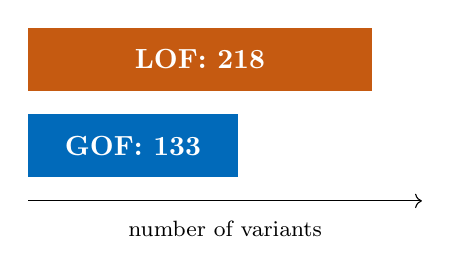
\begin{tikzpicture}
  % LOF bar
  \fill[lofcolor] (0,0) rectangle (4.36,0.8);
  \node[white] at (2.18,0.4) {\textbf{LOF: 218}};
  % GOF bar
  \fill[gofcolor] (0,-1.1) rectangle (2.66,-0.3);
  \node[white] at (1.33,-0.7) {\textbf{GOF: 133}};
  % axis
  \draw[->] (0,-1.4) -- (5,-1.4);
  \node[font=\footnotesize] at (2.5,-1.75) {number of variants};
\end{tikzpicture}\\[0.4cm]
\footnotesize Imbalance $\rightarrow$ \textbf{macro-F1} + stratified CV,
not plain accuracy.
\end{column}
\end{columns}
\end{frame}

% =====================================================================
\begin{frame}{Feature Engineering}
Variant $\rightarrow$ \textbf{52-dim} vector, \textbf{4 groups}:
\vspace{0.2cm}
\begin{table}
\centering
\small
\begin{tabular}{@{}llc@{}}
\toprule
\textbf{Group} & \textbf{What it captures} & \textbf{\# Feat.} \\
\midrule
Physicochemical & 8 AAIndex scales $\times$ \{WT, variant, $\Delta$\} & 24 \\
Substitution    & BLOSUM62 (raw + norm.) + Grantham & 3 \\
Positional      & Normalised position + subunit one-hot (16) & 17 \\
Structural      & RSA, B-factor, DSSP, C$\beta$ density, HSE & 8 \\
\midrule
\textbf{Total}  & & \textbf{52} \\
\bottomrule
\end{tabular}
\caption{Feature groups (also enables ablation studies).}
\end{table}
\footnotesize Interpretable, biologically motivated --- no black-box embeddings.
\end{frame}

% =====================================================================
\begin{frame}{Physicochemical Features (24)}
\begin{columns}[T]
\begin{column}{0.55\textwidth}
\textbf{What}
\begin{itemize}\setlength\itemsep{0.5em}
  \item Captures \textbf{chemistry change} of the swap
  \item \textbf{8 scales} $\times$ \{WT, variant, $\Delta$\} = \textbf{24}
  \item $\Delta$ = variant $-$ wild-type
        \begin{itemize}
          \item size + direction of change
        \end{itemize}
\end{itemize}
\end{column}
\begin{column}{0.45\textwidth}
\small
\textbf{The 8 scales}
\begin{itemize}\setlength\itemsep{0.15em}
  \item Hydrophobicity
  \item Polarity
  \item Volume / size
  \item Molecular weight
  \item Charge (at pH 7)
  \item Isoelectric point
  \item Aromaticity
  \item Secondary-structure preference
\end{itemize}
\end{column}
\end{columns}
\end{frame}

% =====================================================================
\begin{frame}{Substitution Features (3)}
\textbf{How rare / unusual is the swap?}
\medskip
\begin{itemize}\setlength\itemsep{0.5em}
  \item \textbf{BLOSUM62 (raw)} --- evolutionary log-odds score
        \begin{itemize}
          \item high = conservative
          \item negative = disruptive
        \end{itemize}
  \item \textbf{BLOSUM62 (normalised)} --- rescaled to $[0,1]$
  \item \textbf{Grantham distance} --- chemical distance
        \begin{itemize}
          \item $0$ = identical
          \item $215$ = most extreme (Cys $\leftrightarrow$ Trp)
        \end{itemize}
\end{itemize}
\medskip
\footnotesize\emph{Low BLOSUM / high Grantham $\rightarrow$ more drastic swap.}
\end{frame}

% =====================================================================
\begin{frame}{Positional Features (17)}
\begin{columns}[T]
\begin{column}{0.56\textwidth}
\textbf{What}
\begin{itemize}\setlength\itemsep{0.5em}
  \item \textbf{Where} + \textbf{which subunit}
  \item \textbf{Normalised position} (1): scaled to $[0,1]$
  \item \textbf{Subunit one-hot} (16): which nAChR subunit
        \begin{itemize}
          \item CHRNA1--10, CHRNB1--4, CHRND/E/G
        \end{itemize}
  \item Total: \textbf{17}
\end{itemize}
\end{column}
\begin{column}{0.44\textwidth}
\textbf{Why it matters}
\begin{itemize}\setlength\itemsep{0.5em}
  \item Critical regions cluster (pore, ligand-binding)
  \item LOF / GOF differ \emph{by subunit}
\end{itemize}
\end{column}
\end{columns}
\end{frame}

% =====================================================================
\begin{frame}{Structural Features (8)}
\begin{columns}[T]
\begin{column}{0.55\textwidth}
\textbf{What}
\begin{itemize}\setlength\itemsep{0.5em}
  \item \textbf{Per-residue descriptors:}
        \begin{itemize}
          \item RSA (solvent exposure)
          \item B-factor (flexibility)
          \item DSSP (helix / sheet / coil)
          \item C$\beta$ density, HSE (packing)
        \end{itemize}
  \item No structure $\rightarrow$ AlphaFold
\end{itemize}
\end{column}
\begin{column}{0.45\textwidth}
\centering
\small
\begin{tabular}{@{}lll@{}}
\toprule
\textbf{PDB} & \textbf{Type} & \textbf{Subunits} \\
\midrule
7QKO & Muscle & A1, B1, D, E, G \\
7EKI & $\alpha$7 homomer & A7 \\
6CNJ & $\alpha4\beta2$ & A4, B2 \\
6PV7 & $\alpha3\beta4$ & A3, B4 \\
\bottomrule
\end{tabular}
\\[0.3cm]
\footnotesize 6 neuronal subunits $\rightarrow$ AlphaFold.
\end{column}
\end{columns}
\end{frame}

% =====================================================================

\begin{frame}{Pipeline Overview}
\centering
\resizebox{\textwidth}{!}{%
\begin{tikzpicture}[
   node distance=0.6cm and 0.7cm,
   box/.style={rectangle, rounded corners, draw=hbrsblue, very thick,
               fill=hbrsblue!8, text width=2.5cm, align=center,
               minimum height=1.7cm, font=\small},
   arrow/.style={-{Stealth[length=3mm]}, hbrsblue, very thick}]

  \node[box] (data)  {\textbf{Data}\\ curated nAChR\\ variant DB};
  \node[box, right=of data]  (feat)  {\textbf{Features}\\ 52 engineered\\ descriptors};
  \node[box, right=of feat]  (model) {\textbf{Models}\\ LR, SVM, RF,\\ LightGBM};
  \node[box, right=of model] (cv)    {\textbf{Nested CV}\\ 5$\times$5 folds,\\ 5 seeds, Optuna};
  \node[box, right=of cv, fill=gofcolor!15] (pred)
        {\textbf{Prediction}\\ \textcolor{lofcolor}{LOF} /
         \textcolor{gofcolor}{GOF}};

  \draw[arrow] (data)  -- (feat);
  \draw[arrow] (feat)  -- (model);
  \draw[arrow] (model) -- (cv);
  \draw[arrow] (cv)    -- (pred);
\end{tikzpicture}}
\end{frame}

% =====================================================================
\begin{frame}{Methodology}
\begin{columns}[T]
\begin{column}{0.52\textwidth}
\small
\textbf{Models benchmarked}
\begin{itemize}\setlength\itemsep{0.3em}
  \item Logistic Regression
  \item Support Vector Machine (RBF)
  \item Random Forest
  \item LightGBM (gradient boosting)
\end{itemize}
\medskip
\textbf{Evaluation}
\begin{itemize}\setlength\itemsep{0.3em}
  \item \textbf{Nested CV}: 5 outer $\times$ 5 inner
  \item Tuning: \textbf{Optuna} 
  \item $\times$ \textbf{5 seeds}
  \item Metric: \textbf{macro-F1} (imbalance-aware)
\end{itemize}
\end{column}
\begin{column}{0.48\textwidth}
\centering
\begin{tikzpicture}[scale=0.9,
   ofold/.style={rectangle, draw=hbrsblue, very thick, fill=hbrsblue!8,
                 minimum width=4.2cm, minimum height=0.55cm, font=\footnotesize},
   ifold/.style={rectangle, draw=lofcolor, fill=lofcolor!12,
                 minimum width=0.7cm, minimum height=0.4cm, font=\tiny}]
  \node[ofold] (o1) at (0,2.2)  {Outer fold: tune \& test};
  \node[ofold] (o2) at (0,1.5)  {Outer fold};
  \node[ofold] (o3) at (0,0.8)  {Outer fold};
  \node[ofold] (o4) at (0,0.1)  {Outer fold};
  \node[ofold] (o5) at (0,-0.6) {Outer fold};
  \node[font=\footnotesize] at (0,-1.25) {$\times$ 5 seeds};
  \draw[->,hbrsblue,thick] (2.3,0.8) -- (3.2,0.8);
  \node[align=center,font=\footnotesize] at (4.2,0.8)
       {Inner CV\\ + Optuna\\ tuning};
\end{tikzpicture}
\end{column}
\end{columns}
\end{frame}

% =====================================================================
\begin{frame}{Data Augmentation: Mining Mouse Variants}
\textbf{Problem:} human variants scarce ($n = 351$)
\vspace{0.2cm}
\begin{tikzpicture}[
   node distance=0.9cm,
   sbox/.style={rectangle, rounded corners, draw=hbrsblue, very thick,
                fill=hbrsblue!8, text width=3.0cm, align=center,
                minimum height=1.5cm, font=\small},
   arrow/.style={-{Stealth[length=3mm]}, hbrsblue, very thick}]
  \node[sbox] (search) {\textbf{Search}\\ PubMed + Europe PMC\\ ($\sim$5{,}200 papers)};
  \node[sbox, right=of search] (triage) {\textbf{Triage}\\ auto / review / exclude};
  \node[sbox, right=of triage] (extract) {\textbf{Extract}\\ LLM full-text\\ $\rightarrow$ variant rows};
  \draw[arrow] (search) -- (triage);
  \draw[arrow] (triage) -- (extract);
\end{tikzpicture}
\vspace{0.3cm}
\begin{itemize}\setlength\itemsep{0.5em}
  \item \textbf{Mouse} electrophysiology variants 
        
  \item \textbf{Note:} mouse $\neq$ human numbering $\rightarrow$ align first
\end{itemize}
\end{frame}

% =====================================================================
{
\begin{frame}[plain]
\centering
\vfill
{\Huge \textcolor{hbrsblue}{\textbf{Thank you!}}}\\[0.6cm]
{\LARGE \textcolor{hbrsblue}{Questions?}}
\vfill
\end{frame}
}

\end{document}
